\section{Grasping}

In figure~\ref{fig:TouchEgg}, we observe an example of the
compliant sensors working. In this case, the fingers of the hand
close until contact is detected. We see that the sensitivity of
the tactile sensors is enough to detect the contact with an egg
and avoid the fingers to exert excessive force to break it. It is
important to note that the sensors conform to the egg which helps
to constrain the egg's motion and distributes the force reducing
the pressure on the egg's surface.

In order to contrast our compliant sensor features, we refer to
the sensor developed by
Maheshwari~and~Saraf~\cite{touchsensorScience}. This sensor is
capable of recovering the shape embossed on a US penny, but it is
not capable of conforming to the egg. Moreover, given that it is
flat and rigid, the force applied concentrates in a small area
which causes great stress in that area. As reference, this sensor
needs at least $9KPa$ to detect contact. This stress can cause a
fracture on the egg surface.

We further evaluate the compliant sensors on a more delicate task.
In figure~\ref{fig:PaperGentle}, we observe the robot gently
gripping a paper cylinder while the cylinder is only slightly
deformed. There is a weight on the base to keep the cylinder in
place. The weight's size is smaller than the circle of the base so
it does not affect the cylinder structure. The robot's hand
approaches the cylinder by the side. Once the tactile sensors
detect the contact, the robot rotates its finger and closes the
thumb slowly up until contact is detected. The sensitivity of the
compliant tactile sensor is such that the cylinder is only
slightly deformed. On the other hand, we can observe in
figure~\ref{fig:PaperNoGentle} that the cylinder is deformed when
no tactile feedback is used.

The sensitivity of our compliant tactile sensor is in general high
because of its structural design. We can think of the overall
shape of the sensor as an hemisphere, therefore, when the sensor
first comes in contact with a locally flat surface only a point
-in theory- is touched. The stress in that point is high causing
the structure to deform making detection possible. This feature,
allows the sensor to work well with most surfaces.

In contrast, the flat rigid surface of the sensor previously
mentioned~\cite{touchsensorScience} distributes the force applied.
For example, if this sensor comes in contact with a flat surface
of the same size as the sensor's surface, a large force will be
needed to detect the contact. The experiment with the paper
cylinder has little likelihood to work with this sensor, because
the rigidity of its surface will deform the cylinder without
detection.

The sensitivity of the sensor is within the range of human
sensitivity. Human sensitivity is around 0.3~N to 1.0~N as
mentioned in ~\cite{touchsensorScience} and our tactile sensor's
minimum detectable normal force is around 0.1~N in the magnetic
version and 0.01~N in the optical.


Science Paper... Many tactile sensors have only been tested on the
bench. Focus on get density... However, no much attention to the
data produced. We for example believe that those properties are
important but not as much as the shape.
%


\begin{figure}[tbp]
\centerline{
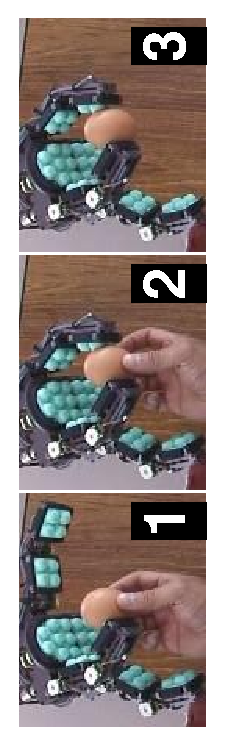
\includegraphics[height=\columnwidth, angle=270 ]{./figures/EggSeq.eps}
} \caption[Grabbing an egg]{In this sequence we observe the hand
closing on a egg. This task is easier than the one shown in
figure~\ref{fig:PaperGentle}. If we observe carefully 3. we can
notice the properties of the tactile sensors. They detect the
contact but also conform to the object increasing friction and
making an stable grasp possible.} \label{fig:TouchEgg}
\end{figure}

\begin{figure}[tbp]
\centerline{
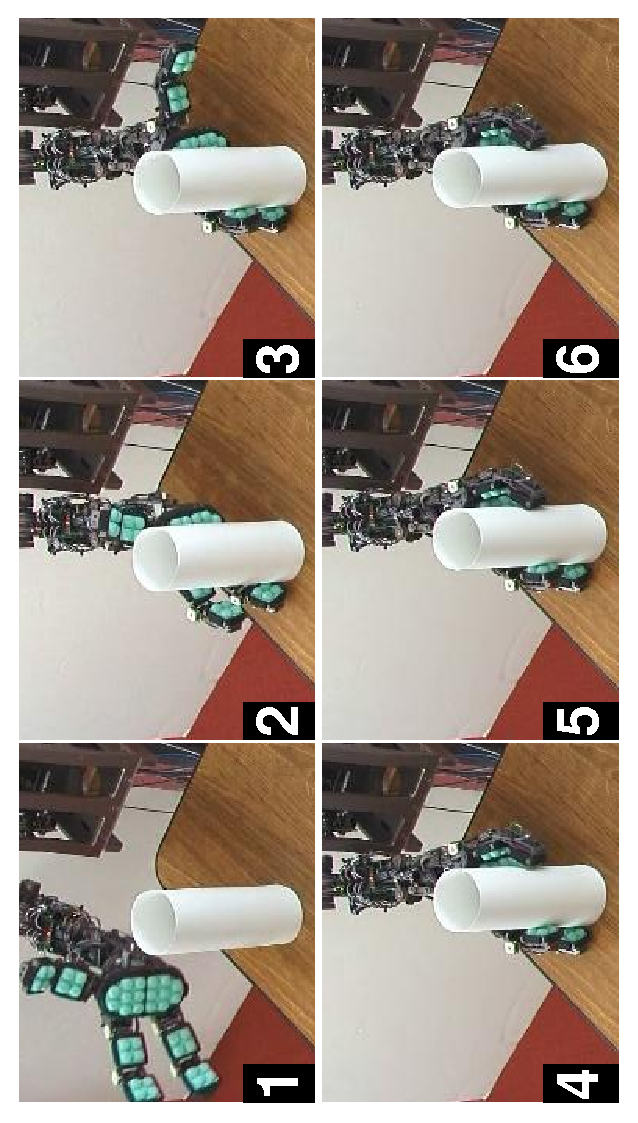
\includegraphics[height=\columnwidth, angle=270 ]{./figures/PaperGentle.eps}
} \caption[Gently grabbing a paper cylinder]{In this sequence we
observe the robot approaching a cylinder made of paper bond. This
cylinder has a weight in its bottom. The robot can detect the
first contact, oppose its thumb and move the thumb, gently
stopping when detecting the contact. The tactile sensors are
sensitive enough to detect the cylinder without crushing it.}
\label{fig:PaperGentle}
\end{figure}

\begin{figure}[tbp]
\centerline{
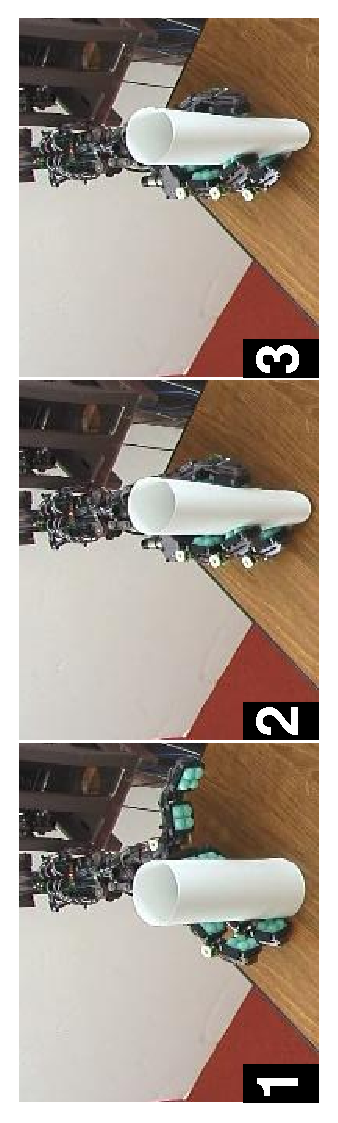
\includegraphics[height=\columnwidth, angle=270 ]{./figures/PaperNoGentle.eps}
} \caption[Crushing paper cylinder]{In this sequence the robot
closes its fingers without using tactile feedback. As a
consequence they crush the object.} \label{fig:PaperNoGentle}
\end{figure}



